In type theory and categorical logic, the idea of multicategories is to give
an algebraic structure that is close to the syntax of type theory.
In simple type theory, sequents take the form $\Gamma \vdash A$, where $A$ is
the type of the conclusion and $\Gamma$ is a list of types, one type for each
assumption.
Intuitively, a term with assumptions $\Gamma$ and type $A$ constitutes a
morphism from $\Gamma$ to $A$.
Multicategories make this structure --- domains being lists of objects and
codomains being a single object --- part of the definition of morphisms.

\begin{definition}[multicategory]
  A \emph{multicategory} comprises a collection of objects $\obj$, for each
  list of objects $\Gamma$ and object $A$ a set of (multi)morphisms
  $\hom(\Gamma, A)$, and the following morphisms, satisfying the following
  axioms.

  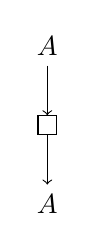
\begin{tikzpicture}
    \path
    (0,1) node(s) {$A$}
    (0,0) node[draw](id) {$\id$}
    (0,-1) node(t) {$A$}
    ;

    \draw[->] (s) -- (id);
    \draw[->] (id) -- (t);
  \end{tikzpicture}
  \begin{tikzpicture}
    \path
    (-2,2) node(A11) {$A_{11}$}
    (-1.5,1.5) node(A1dots) {$\cdots$}
    (-1,2) node(A1n) {$A_{1n}$}
    (0,2) node(Adots) {$\cdots$}
    (1,2) node(Am1) {$A_{m1}$}
    (1.5,1.5) node(Amdots) {$\cdots$}
    (2,2) node(Amn) {$A_{mn}$}

    (-1.5,1) node[draw](f1) {$f_1$}
    (0,1) node(fdots) {$\cdots$}
    (1.5,1) node[draw](fm) {$f_m$}

    (0,0) node[draw](g) {$g$}

    (0,-1) node(C) {$C$}
    ;

    \node[draw,dotted,fit=(f1) (fm) (g),
    label=below right:{\footnotesize$g \circ (f_1, \ldots, f_m)$}] (box) {};

    \draw[->] (A11) -- (f1);
    \draw[->] (A1n) -- (f1);
    \draw[->] (Am1) -- (fm);
    \draw[->] (Amn) -- (fm);
    \draw[->] (f1) -- (g);
    \draw[->] (fm) -- (g);
    \draw[->] (g) -- (C);
  \end{tikzpicture}

  \begin{displaymath}
    \begin{matrix}
      \begin{tikzpicture}[baseline]
        \path
        (-1,2) node(A1) {$A_1$}
        (0,2) node(Adots) {$\cdots$}
        (1,2) node(An) {$A_n$}
        (0,1) node[draw](f) {$f$}
        (0,0) node[draw](id) {$\id$}
        (0,-1) node(t) {$A$}
        ;

        \node[draw,dotted,fit=(f) (id)] {};

        \draw[->] (A1) -- (f);
        \draw[->] (An) -- (f);
        \draw[->] (f) -- (id);
        \draw[->] (id) -- (t);
      \end{tikzpicture}
      =
      \begin{tikzpicture}[baseline]
        \path
        (-1,1) node(A1) {$A_1$}
        (0,1) node(Adots) {$\cdots$}
        (1,1) node(An) {$A_n$}
        (0,0) node[draw](f) {$f$}
        (0,-1) node(t) {$A$}
        ;

        \draw[->] (A1) -- (f);
        \draw[->] (An) -- (f);
        \draw[->] (f) -- (t);
      \end{tikzpicture}
      &\phantom{mmmm}&
      \begin{tikzpicture}[baseline]
        \path
        (-1,2) node(A1) {$A_1$}
        (0,2) node(Adots) {$\cdots$}
        (1,2) node(Am) {$A_m$}
        (-1,1) node[draw](id1) {$\id$}
        (0,1) node(iddots) {$\cdots$}
        (1,1) node[draw](idm) {$\id$}
        (0,0) node[draw](f) {$f$}
        (0,-1) node(t) {$A$}
        ;

        \node[draw,dotted,fit=(id1) (idm) (f)] {};

        \draw[->] (A1) -- (id1);
        \draw[->] (Am) -- (idm);
        \draw[->] (id1) -- (f);
        \draw[->] (idm) -- (f);
        \draw[->] (f) -- (t);
      \end{tikzpicture}
      =
      \begin{tikzpicture}[baseline]
        \path
        (-1,1) node(A1) {$A_1$}
        (0,1) node(Adots) {$\cdots$}
        (1,1) node(An) {$A_n$}
        (0,0) node[draw](f) {$f$}
        (0,-1) node(t) {$A$}
        ;

        \draw[->] (A1) -- (f);
        \draw[->] (An) -- (f);
        \draw[->] (f) -- (t);
      \end{tikzpicture}
    \end{matrix}
  \end{displaymath}

  \begin{displaymath}
    \begin{matrix}
      \begin{tikzpicture}
        \path
        % left
        (-5,2) node(A111) {$A_{111}$}
        (-4.5,1.5) node(A1dots) {$\cdots$}
        (-4,2) node(A11n) {$A_{11n}$}
        (-3,2) node(Adots) {$\cdots$}
        (-2,2) node(A1m1) {$A_{1m1}$}
        (-1.5,1.5) node(Amdots) {$\cdots$}
        (-1,2) node(A1mn) {$A_{1mn}$}

        (-4.5,1) node[draw](f11) {$f_{11}$}
        (-3,1) node(fdots) {$\cdots$}
        (-1.5,1) node[draw](f1m) {$f_{1m}$}

        (-3,0) node[draw](g1) {$g_1$}

        % right
        (1,2) node(Al11) {$A_{l11}$}
        (1.5,1.5) node(A1dots) {$\cdots$}
        (2,2) node(Al1n) {$A_{l1n}$}
        (3,2) node(Adots) {$\cdots$}
        (4,2) node(Alm1) {$A_{lm1}$}
        (4.5,1.5) node(Amdots) {$\cdots$}
        (5,2) node(Almn) {$A_{lmn}$}

        (1.5,1) node[draw](fl1) {$f_{l1}$}
        (3,1) node(fdots) {$\cdots$}
        (4.5,1) node[draw](flm) {$f_{lm}$}

        (3,0) node[draw](gl) {$g_l$}

        % middle
        (0,2) node {$\cdots$}
        (0,0.5) node {$\cdots$}
        (0,-1) node[draw](h) {$h$}
        (0,-2) node(D) {$D$}
        ;

        \node[draw,dotted,fit=(f11) (f1m) (g1)] (box1) {};
        \node[draw,dotted,fit=(fl1) (flm) (gl)] (boxl) {};
        \node[draw,dotted,fit=(box1) (boxl) (h)] (box) {};

        \draw[->] (A111) -- (f11);
        \draw[->] (A11n) -- (f11);
        \draw[->] (A1m1) -- (f1m);
        \draw[->] (A1mn) -- (f1m);
        \draw[->] (f11) -- (g1);
        \draw[->] (f1m) -- (g1);
        \draw[->] (g1) -- (h);

        \draw[->] (Al11) -- (fl1);
        \draw[->] (Al1n) -- (fl1);
        \draw[->] (Alm1) -- (flm);
        \draw[->] (Almn) -- (flm);
        \draw[->] (fl1) -- (gl);
        \draw[->] (flm) -- (gl);
        \draw[->] (gl) -- (h);

        \draw[->] (h) -- (D);
      \end{tikzpicture}
      \\=\\
      \begin{tikzpicture}
        \path
        % left
        (-5,2) node(A111) {$A_{111}$}
        (-4.5,1.5) node(A1dots) {$\cdots$}
        (-4,2) node(A11n) {$A_{11n}$}
        (-3,2) node(Adots) {$\cdots$}
        (-2,2) node(A1m1) {$A_{1m1}$}
        (-1.5,1.5) node(Amdots) {$\cdots$}
        (-1,2) node(A1mn) {$A_{1mn}$}

        (-4.5,1) node[draw](f11) {$f_{11}$}
        (-3,1) node(fdots) {$\cdots$}
        (-1.5,1) node[draw](f1m) {$f_{1m}$}

        (-3,0) node[draw](g1) {$g_1$}

        % right
        (1,2) node(Al11) {$A_{l11}$}
        (1.5,1.5) node(A1dots) {$\cdots$}
        (2,2) node(Al1n) {$A_{l1n}$}
        (3,2) node(Adots) {$\cdots$}
        (4,2) node(Alm1) {$A_{lm1}$}
        (4.5,1.5) node(Amdots) {$\cdots$}
        (5,2) node(Almn) {$A_{lmn}$}

        (1.5,1) node[draw](fl1) {$f_{l1}$}
        (3,1) node(fdots) {$\cdots$}
        (4.5,1) node[draw](flm) {$f_{lm}$}

        (3,0) node[draw](gl) {$g_l$}

        % middle
        (0,2) node {$\cdots$}
        (0,1) node {$\cdots$}
        (0,0) node {$\cdots$}
        (0,-1) node[draw](h) {$h$}
        (0,-2) node(D) {$D$}
        ;

        \node[draw,dotted,fit=(g1) (gl) (h)] (boxi) {};
        \node[draw,dotted,fit=(f11) (f1m) (fl1) (flm) (boxi)] (boxo) {};

        \draw[->] (A111) -- (f11);
        \draw[->] (A11n) -- (f11);
        \draw[->] (A1m1) -- (f1m);
        \draw[->] (A1mn) -- (f1m);
        \draw[->] (f11) -- (g1);
        \draw[->] (f1m) -- (g1);
        \draw[->] (g1) -- (h);

        \draw[->] (Al11) -- (fl1);
        \draw[->] (Al1n) -- (fl1);
        \draw[->] (Alm1) -- (flm);
        \draw[->] (Almn) -- (flm);
        \draw[->] (fl1) -- (gl);
        \draw[->] (flm) -- (gl);
        \draw[->] (gl) -- (h);

        \draw[->] (h) -- (D);
      \end{tikzpicture}
    \end{matrix}
  \end{displaymath}
\end{definition}

Multicategories have been used as a framework for reasoning with multilinear
maps in linear algebra. \todo{Reference?}
We can produce a multicategory where the objects are vector spaces, and the
multimorphisms are multilinear maps.
In this setting, we can give a universal property to the tensor product of
vector spaces.

\begin{definition}[tensor product \& tensor unit]
  Given a multicategory $\C$, a \emph{tensor product} in $\C$ is a function
  ${\otimes} : \obj\C \times \obj\C \to \obj\C$ and for each pair of objects
  $A$ and $B$, a multimorphism ${\otimes} : A, B \to A \otimes B$ such that,
  for any multimorphism $f : A, B \to C$, there is a unique way to factor $f$
  through $\otimes$, as shown below.
  Similarly, a \emph{tensor unit} is an object $I$ of $\C$ and a multimorphism
  $I : \varepsilon \to I$ supporting a nullary unique factorisation.

  \begin{tikzcd}
    A, B \arrow[rd,"f"'] \arrow[r,"\otimes"] & A \otimes B \arrow[d, dashed] \\
    & C
  \end{tikzcd}
  \begin{tikzcd}
    \varepsilon \arrow[rd,"f"'] \arrow[r,"I"] & I \arrow[d, dashed] \\
    & C
  \end{tikzcd}
\end{definition}

As the proliferation of ellipses suggests, the definition of
\emph{multicategory} I gave above is not entirely rigorous.
Indeed, mechanising the multicategory definition in a reasonably usable way is
considered an open problem. \todo{Check that no-one has done it}
However, we \emph{can} achieve a simple and usable definition in the special
case of \emph{Cartesian} multicategories.

Ordinary multicategories are to monoidal categories as Cartesian multicategories
are to Cartesian categories (i.e., categories with all finite products).
Cartesian multicategories can be defined in terms of ordinary multicategories
--- they are multicategories satisfying the usual ``structural rules'' below
and satisfying various coherence conditions on them.

\begin{align*}
  e &: \hom(\Gamma, A, B, \Delta; C) \to \hom(\Gamma, B, A, \Delta; C) \\
  w &: \hom(\Gamma; B) \to \hom(\Gamma, A; B) \\
  c &: \hom(\Gamma, A, A; B) \to \hom(\Gamma, A; B)
\end{align*}

However, we can bypass ordinary multicategories entirely, and give the following
definition inspired by our earlier formulation of intuitionistic logic.
I define Cartesian multicategories in tandem with the category of contexts and
substitutions that a Cartesian multicategory yields.

\begin{definition}
  A \emph{Cartesian multicategory} comprises the following.

  \begin{itemize}
    \item We have a collection of objects $\obj$.
          We call a list of objects a \emph{context}.
    \item For each context $\Gamma$ and object $A$, we have a set of
          (multi)morphisms $\hom(\Gamma; A)$.
          From this, we derive, for any contexts $\Gamma$ and $\Delta$, a set
          of \emph{substitutions}
          $\sub(\Gamma; \Delta) \coloneqq \prod X \in \Delta.~\hom(\Gamma; X)$.
    \item For every $i : A \in \Gamma$, we have an identity morphism
          $\id(i) : \hom(\Gamma; A)$.
          The collection of identity morphisms over $\Gamma$ serves as the
          identity substitution $\id^s : \sub(\Gamma; \Gamma)$.
    \item For substitution $\sigma : \sub(\Gamma; \Delta)$ and morphism
          $f : \hom(\Delta; A)$, we get a composite morphism
          $\sigma ; f : \hom(\Gamma; A)$.
          This allows us to compose substitutions; for
          $\sigma : \sub(\Gamma; \Delta)$ and $\tau : \sub(\Delta; \Theta)$,
          let $\sigma;^s \tau \coloneqq \lambda k.~\sigma; \tau(k)$.
    \item Identity and composition satisfy the following laws.
          \begin{itemize}
            \item $\sigma; \id(i) = \sigma(i)$
            \item $\id^s; f = f$
            \item $(\sigma;^s \tau); f = \sigma; (\tau; f)$
          \end{itemize}
          It is a simple exercise to see that these laws exactly give us the
          category laws of identity and associativity for substitutions.
  \end{itemize}
\end{definition}

The category of contexts and substitutions is furthermore Cartesian, with the
product being given by context concatenation.
